\section{Globaal ontwerp}  \label{sec:globaal}
Canvas.hs is een library die de programmeur kan importeren in zijn programma om er daarna met de API die Canvas.hs aanbiedt gemakkelijk een uitgebreide user interface mee te bouwen. Canvas.hs focust zich op elementaire input en geen ondersteuning heeft voor high level interface elementen zoals buttons en textarea's. Deze elementen zullen\todo{niet eigen systeem afzwakken} met behulp van Canvas.hs wel eenvoudig te implementeren zijn. \autoref{fig:demo_screenshot} geeft een demoapplicatie van Canvas.hs weer.


\begin{figure}[H]
\begin{center}
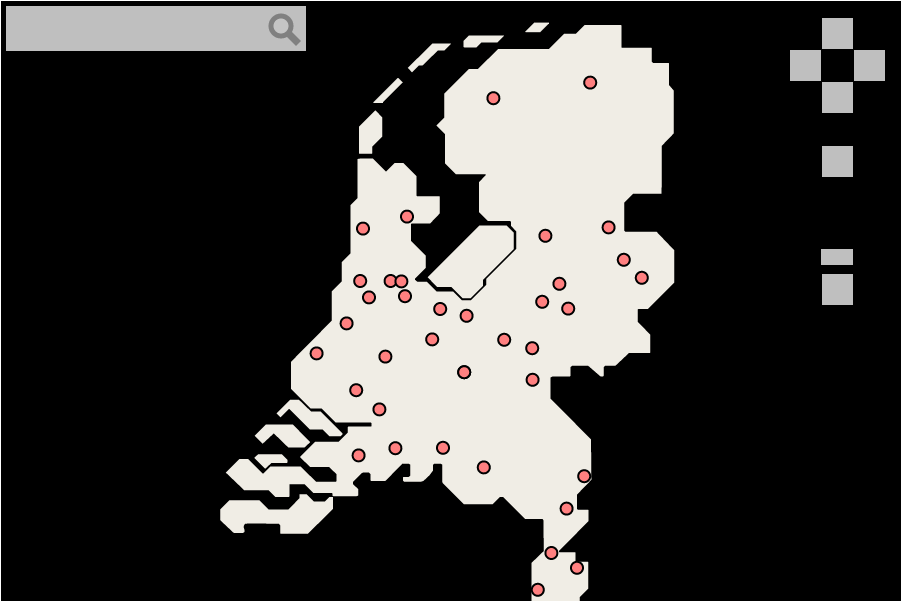
\includegraphics[keepaspectratio,width=\textwidth]{./images/demo.png}
\caption{Een demoapplicatie van de Canvas.hs library}
\label{fig:demo_screenshot}
\end{center}
\end{figure}


\autoref{fig:overzicht_architectuur} geeft een overzicht van de architectuur. Canvas.hs bestaat uit een module en een client. De module is een library die de programmeur in zijn programma importeert. Bij het starten van de module start een HttpServer, een WebSocket-server en wordt de webpagina van de client automatisch gestart. De client bestaat uit een browserpagina met onder andere een canvas element. De module communiceert met de client via een WebSocket verbinding om grafische elementen op de canvas in de client te tekenen.

\begin{figure}[H]
\begin{center}
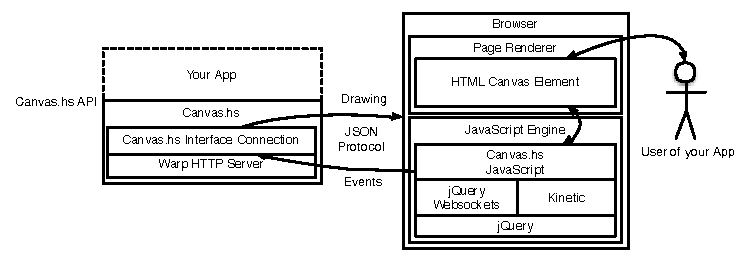
\includegraphics[keepaspectratio,width=\textwidth]{./images/architectuur_overzicht.pdf}
\caption{Overzicht van de architectuur van Canvas.hs}
\label{fig:overzicht_architectuur}
\end{center}
\end{figure}

\todo{uitbreiden over shapes}
\todo{uitbreiden met een klein stukje voorbeeldCode en wat meer uitleg over type v.d. eventHandler}
\todo{aanpasssen dat we meer uitleg over het concept hebben, zodat veel termen niet in het detailontwerp voor het eerst langskomen. Het detailontwerp leest nu teveel als een globaalontwerp met allemaal ontwerpkeuzes erdoorheen gestrooid, kort vertellen over gebruik libries als KineticJS e.d.}

Canvas.hs roept de eventhandler van de gebruiker aan met alle events die er in de grafische interface gebeuren. De eventhandler krijgt het event en de huidige state variabele als parameters mee en moet daarop de nieuwe state variabele en output teruggeven. Output bestaat uit acties die op de client uitgevoerd kunnen worden (zoals een prompt, fullscreen of download) en grafische output in de vorm van shapes.
